\documentclass[a4paper]{deedy-resume} % Use US Letter paper, change to a4paper for A4 

\begin{document}

%----------------------------------------------------------------------------------------
%	TITLE SECTION
%----------------------------------------------------------------------------------------

\lastupdated % Print the Last Updated text at the top right

\namesection{Stefano}{Forti}{ % Your name
\urlstyle{same}\url{http://stefanoforti.altervista.org} \\ % Your website, LinkedIn profile or other web address
\href{mailto:stefano.forti92@gmail.com}{stefano.forti92@gmail.com} | 333 27 18 311 % Your contact information
}

%----------------------------------------------------------------------------------------
%	LEFT COLUMN
%----------------------------------------------------------------------------------------

\begin{minipage}[t]{0.33\textwidth} % The left column takes up 33% of the text width of the page

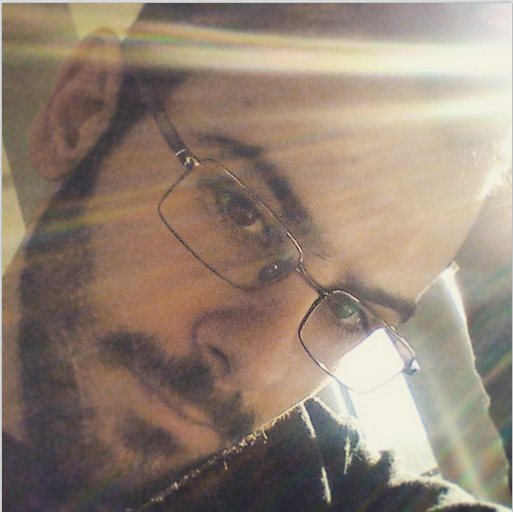
\includegraphics[width=0.5\textwidth]{photo.png}

%------------------------------------------------
% Education
%------------------------------------------------

\section{Educazione} 

\subsection{SSSUP Sant'Anna \& Università di Pisa}

\descript{Laurea Magistrale in Informatica e Networking}
\location{Previsto 2016 | Pisa \\ Media: 28}

\sectionspace % Some whitespace after the section

\subsection{Università di Pisa}

\descript{Laurea Triennale in Informatica}
\location{Settembre 2011 - Luglio 2014 | Pisa}
\location{110 e lode}

\sectionspace % Some whitespace after the section

%------------------------------------------------

\subsection{La Martiniere for Boys}

\location{Grad. May 2011 | Kolkata, India}

\sectionspace % Some whitespace after the section

%------------------------------------------------
% Links
%------------------------------------------------

\section{Links} 

Github:// \href{https://github.com/deedydas}{\bf deedydas} \\
LinkedIn:// \href{https://www.linkedin.com/in/debarghyadas}{\bf debarghyadas} \\
YouTube:// \href{https://www.youtube.com/user/DeedyDash007}{\bf DeedyDash007} \\
Twitter:// \href{https://twitter.com/debarghya_das}{\bf @debarghya\_das} \\
Quora:// \href{https://www.quora.com/Debarghya-Das}{\bf Debarghya-Das}

\sectionspace % Some whitespace after the section

%------------------------------------------------
% Coursework
%------------------------------------------------

\section{Coursework}

\subsection{Graduate}

Advanced Machine Learning \\
Open Source Software Engineering \\
Advanced Interactive Graphics \\
Compilers + Practicum \\
Cloud Computing

\sectionspace % Some whitespace after the section

%------------------------------------------------

\subsection{Undergraduate}

Information Retrieval \\
Operating Systems \\
Artificial Intelligence + Practicum \\
Functional Programming \\
Computer Graphics + Practicum \\
{\footnotesize \textit{\textbf{(Research Asst. \& Teaching Asst) }}} \\
Unix Tools and Scripting

\sectionspace % Some whitespace after the section

%------------------------------------------------
% Skills
%------------------------------------------------

\section{Skills}

\subsection{Programming}

\location{Over 5000 lines:}
Java \textbullet{} Shell \textbullet{} JavaScript \textbullet{} Matlab \\
OCaml \textbullet{} Python \textbullet{} Rails \textbullet{} \LaTeX\ \\ 
\location{Over 1000 lines:}
C \textbullet{} C++ \textbullet{} CSS \textbullet{} PHP \textbullet{} Assembly \\
\location{Familiar:}
AS3 \textbullet{} iOS \textbullet{} Android \textbullet{} MySQL

\sectionspace % Some whitespace after the section

%----------------------------------------------------------------------------------------

\end{minipage} % The end of the left column
\hfill
%
%----------------------------------------------------------------------------------------
%	RIGHT COLUMN
%----------------------------------------------------------------------------------------
%
\begin{minipage}[t]{0.66\textwidth} % The right column takes up 66% of the text width of the page

%------------------------------------------------
% Experience
%------------------------------------------------

\section{Experience}

\runsubsection{Coursera}
\descript{| KPCB Fellow + Software Engineering Intern}

\location{Expected June 2014 – Sep 2014 | Mountain View, CA}
\vspace{\topsep} % Hacky fix for awkward extra vertical space
\begin{tightitemize}
\item 52 out of 2500 applicants chosen to be a KPCB Fellow 2014.
\end{tightitemize}

\sectionspace % Some whitespace after the section

%------------------------------------------------

\runsubsection{Google}
\descript{| Software Engineering Intern}

\location{May 2013 – Aug 2013 | Mountain View, CA}
\begin{tightitemize}
\item Worked on the YouTube Captions team in primarily vanilla Javascript and Python to plan, design and develop the full stack implementation of a new framework to add and edit Automatic Speech Recognition captions.
\item Created a backbone.js-like framework for the Captions editor.
\item All code was reviewed, perfected, and pushed to production.
\end{tightitemize}

\sectionspace % Some whitespace after the section

%------------------------------------------------

\runsubsection{Phabricator}
\descript{| Open Source Contributor \& Team Leader}

\location{Jan 2013 – May 2013 | Palo Alto, CA \& Ithaca, NY}
\begin{tightitemize}
\item Phabricator is used daily by Facebook, Dropbox, Quora, Asana and more.
\item I created the Meme generator, the entire Lipsum application, ported Tokens to different apps, fixed many bugs and more in PHP and Shell.
\item Led a team from MIT, Cornell, IC London and UHelsinki for the project.
\end{tightitemize}

\sectionspace % Some whitespace after the section

%------------------------------------------------
% Research
%------------------------------------------------

\section{Research}

\runsubsection{Cornell Robot Learning Lab}
\descript{| Head Undergrad Research}

\location{Jan 2014 – Present | Ithaca, NY}
Worked with \textbf{\href{http://www.cs.cornell.edu/~ashesh/}{Ashesh Jain}} and \textbf{\href{http://www.cs.cornell.edu/~asaxena/}{Prof Ashutosh Saxena}} to create \textbf{PlanIt}, a tool which learns from large scale user preference feedback to plan robot trajectories in human environments. Publication submitted.

\sectionspace % Some whitespace after the section

%------------------------------------------------

\runsubsection{Cornell Phonetics Lab}
\descript{| Head Undergraduate Researcher}

\location{Mar 2012 – May 2013 | Ithaca, NY}
Lead the development of \textbf{QuickTongue}, the first ever breakthrough tongue-controlled game with \textbf{\href{http://conf.ling.cornell.edu/~tilsen/}{Prof Sam Tilsen}} to aid in Linguistics research. Publication submitted.

\sectionspace % Some whitespace after the section

%------------------------------------------------
% Awards
%------------------------------------------------

\section{Awards} 

\begin{tabular}{rll}
2014	 & top 52/2500 & KPCB Engineering Fellow\\
2014	 & 2\textsuperscript{nd} most points & Google Code Jam, Qualification Round\\
2014	 & 1\textsuperscript{st}/50 & Microsoft Coding Competition, Cornell\\
2013	 & National & Jump Trading Challenge Finalist\\
2013 & 7\textsuperscript{th}/120 & CS 3410 Cache Race Bot Tournament \\
2012 & 2\textsuperscript{nd}/150 & CS 3110 Biannual Intra-Class Bot Tournament \\
2011 & National & Indian National Mathematics Olympiad (INMO) Finalist \\
2010 & National & Comp. Soc. of India's National Programming Contest\\
\end{tabular}

\sectionspace % Some whitespace after the section

%------------------------------------------------
% Societies
%------------------------------------------------

\section{Societies} 

\begin{tabular}{rll}
2014 & top 12\%ile & Tau Beta Pi Engineering Honor Society\\
2014 & National & The Global Leadership and Education Forum (tGELF)\\
2012 & National & Golden Key International Honor Society\\
2012 & National & National Society of Collegiate Scholars\\
\end{tabular}

\sectionspace % Some whitespace after the section

%----------------------------------------------------------------------------------------

\end{minipage} % The end of the right column

%----------------------------------------------------------------------------------------
%	SECOND PAGE (EXAMPLE)
%----------------------------------------------------------------------------------------

%\newpage % Start a new page

%\begin{minipage}[t]{0.33\textwidth} % The left column takes up 33% of the text width of the page

%\section{Example Section}

%\end{minipage} % The end of the left column
%\hfill
%\begin{minipage}[t]{0.66\textwidth} % The right column takes up 66% of the text width of the page

%\section{Example Section 2}

%\end{minipage} % The end of the right column

%----------------------------------------------------------------------------------------

\end{document}